\documentclass[11pt]{article}

\usepackage{times}
\usepackage{alltt}
\usepackage{exam}
\usepackage{graphicx} 
\usepackage{wrapfig} 

%%%%%%%%%%%%%% 
%% Page layout
%%%%%%%%%%%%%%
\oddsidemargin 0pt
\evensidemargin 0pt
\textheight 600pt
\textwidth 469pt
\setlength{\parindent}{0em}
\setlength{\parskip}{1ex}

\begin{document}
\begin{flushright}
{\large\bf Full Name:\_\_\_\_\_\_\_\_\_\_\_\_\_\_\_\_\_\_\_\_\_\_\_\_\_\_\_\_\_\_\_\_\_\_\_\_\_\_\_\_\_ } \\[1ex]
\end{flushright}
\vspace*{0.5 in}

\setcounter{maxpage}{8}

\begin{center}
{\LARGE\bf CS 4300, Fall 2018\\ [2 ex]
Written Exam I}\\ [2 ex]
Sep 27, 2018
\end{center}

\textbf{Scenario 1}

The intersection of University Avenue and St. George Boulevard handles a lot of traffic,
both vehicles and pedestrians.  Traffic lights, including crosswalk lights, control the flow of traffic.
There are crosswalks for all four crossing directions.  Our agent is located on the
south-east corner of the intersection and needs to reach the north-west corner.
The agent is a physical machine, about 3 feet tall with a doom shaped top.  
The agent has audio and visual sensors, and motion actuators that allow the agent to move
forward and rotate to change direction. The agent carries vital information that must
reach the north-west corner to save the inhabitants of Washington County from
a life of oppression.

\begin{problem}{2}
  Describe the performance measure you would use for this environment. Explain each term of the formula.
  \vspace*{1.5in}
\end{problem}

\begin{problem}{2}
  What are the important percepts a software developer would want to derive from the sensors?
  \vspace*{1in}
\end{problem}

\begin{problem}{2}
  What are the important actions a software developer would want to use from the actuators?
  \vspace*{1in}
\end{problem}

\begin{problem}{2}
  Would you classify this environment as Fully or Partially Observable? Why?
  \vspace*{1in}
\end{problem}

\begin{problem}{2}
  Would you classify this environment as Episodic or Sequential? Why?
  \vspace*{1in}
\end{problem}

\begin{problem}{2}
  Would you classify this environment as Deterministic or Stochastic? Why?
  \vspace*{1in}
\end{problem}

\begin{problem}{2}
  Would you classify this environment as Static or Dynamic? Why?
  \vspace*{1in}
\end{problem}

\begin{problem}{2}
  Would you classify this environment as Single or Multi Agent? Why?
  \vspace*{1in}
\end{problem}

\begin{problem}{2}
  Would you classify this environment as Discrete or Continuous? Why?
  \vspace*{1in}
\end{problem}

\begin{problem}{2}
  Would you classify this environment as Known or Unknown? Why?
  \vspace*{1in}
\end{problem}

\begin{problem}{2}
  What type of agent implementation (e.g. Reflex, Model, Goal, Utility, etc.) would you choose to create an agent that would perform well in this environment?  Why?
  \vspace*{1in}
\end{problem}


\newpage
\textbf{Scenario 2}

\begin{wrapfigure}{R}{0.20\textwidth}
  \vspace{-22pt}
  \begin{center}
    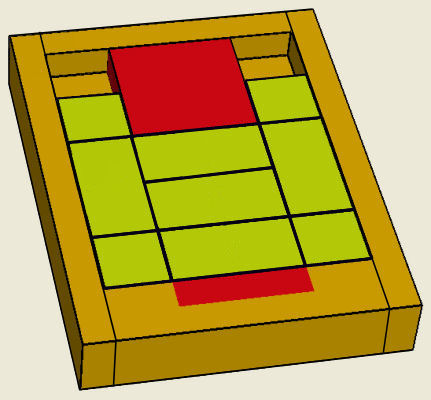
\includegraphics[width=0.20\textwidth]{jk-supercompo.jpg}
  \end{center}
  \vspace{-20pt}
  \caption{Supercompo Puzzle}
\end{wrapfigure}

The puzzle shown is a variation of slider puzzles.  Legal moves are made
by sliding a piece into an unoccupied area.  Each slide is a separate
move.  In this puzzle, the pieces have a variety of shapes.  The goal
is to move the big red piece to the bottom of the box next to the
red line on the border.  Our agent is a digital agent.  It is presented with
a digital copy of the problem in a suitable format and returns a sequence
of actions in a suitable format.

For this set of problems, consider implementing the Supercompo agent using classic search.
If you don't have sufficient information to answer any question, make your
best guess, and state why you feel it is inaccurate.

\begin{problem}{2}
  What is the maximum value of $b$, the branching factor?  Be sure to consider
  advanced states of the puzzle, not just the start state.
  \vspace*{1in}
\end{problem}

\begin{problem}{2}
  What is the value of $m$, the maximum tree depth?
  \vspace*{1in}
\end{problem}

\begin{problem}{2}
  What is the value of $d$, the depth of the shallowest goal?
  \vspace*{1in}
\end{problem}

\begin{problem}{2}
  Would you use tree or graph search for this problem?  Why?
  \vspace*{1in}
\end{problem}

\begin{problem}{2}
  Which frontier variety (e.g. DFS, DL, IDS, BFS, UC, A*, etc.) would you use?  Why?
  \vspace*{1in}
\end{problem}

\begin{problem}{2}
  Are your choices for the previous two questions consistent? Why?
  \vspace*{1in}
\end{problem}


\newpage
\textbf{Scenario 3}

A particular search problem has no heuristic available, but needs to be solved as efficiently as possible.  Analysis shows that the search tree for the problem is finite with a maximum depth of 10.  Each state has up to 3 legal actions.  The goal states are only found at the maximum depth.  Each problem instance has many goal states;  approximately 50\% of the maximum depth states are goals, spread across the maximum depth.  This search needs to take place on a micro-server, quickly finding its solutions to keep lag times for users minimum.  Each solution needs to be found in less than 0.5 seconds.  Because of the nature of the problem, each node takes approximately 0.001 seconds to expand.  Note: $3^{10} = 59049$.

\begin{problem}{8}

  Write the Big-O limits on the time and space complexity for BFS and DSF on this problem.  Give numbers and the formulas used to calculate them.
  
  \vspace*{1in}
  
\end{problem}

\begin{problem}{2}

  Which classic tree search strategy (not limited to BFS and DFS) would you use for this problem?
  Why?
  
  \vspace*{1in}
  
\end{problem}




\newpage
\textbf{Scenario 4}

Description copied verbatim from Wikipedia.

\begin{wrapfigure}{R}{0.20\textwidth}
  \vspace{-22pt}
  \begin{center}
    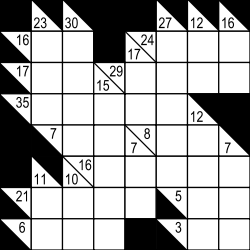
\includegraphics[width=0.20\textwidth]{250px-Kakuro_black_box.png}
  \end{center}
  \vspace{-20pt}
  \caption{Kakuro Puzzle}
\end{wrapfigure}
The canonical Kakuro puzzle is played in a grid of filled and barred cells, "black" and "white" respectively. Puzzles are usually 16×16 in size, although these dimensions can vary widely. Apart from the top row and leftmost column which are entirely black, the grid is divided into "entries"—lines of white cells—by the black cells. The black cells contain a diagonal slash from upper-left to lower-right and a number in one or both halves, such that each horizontal entry has a number in the black half-cell to its immediate left and each vertical entry has a number in the black half-cell immediately above it. These numbers, borrowing crossword terminology, are commonly called "clues".
\begin{wrapfigure}{R}{0.20\textwidth}
  \vspace{-22pt}
  \begin{center}
    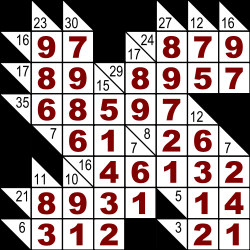
\includegraphics[width=0.20\textwidth]{250px-Kakuro_black_box_solution.png}
  \end{center}
  \vspace{-20pt}
  \caption{Kakuro Solution}
\end{wrapfigure}

The objective of the puzzle is to insert a digit from 1 to 9 inclusive into each white cell such that the sum of the numbers in each entry matches the clue associated with it and that no digit is duplicated in any entry. It is that lack of duplication that makes creating Kakuro puzzles with unique solutions possible, and which means solving a Kakuro puzzle involves investigating combinations more, compared to Sudoku in which the focus is on permutations. There is an unwritten rule for making Kakuro puzzles that each clue must have at least two numbers that add up to it, since including only one number is mathematically trivial when solving Kakuro puzzles.

For this set of problems, consider implementing the Kakuro agent using local search.
If you don't have sufficient information to answer any question, make your
best guess, and state why you feel it is inaccurate.

\begin{problem}{2}
  Describe a state of this problem.
  \vspace*{1in}
\end{problem}

\begin{problem}{2}
  Assume gradient descent is to be used.  Describe a suitable utility function.
  \vspace*{1in}
\end{problem}

\begin{problem}{2}
  Assume gradient descent is to be used.  Describe the neighbors of a state.
  \vspace*{1in}
\end{problem}

\begin{problem}{2}
  Assume gradient descent is to be used.  Would you expect to need random restart?  Why?
  \vspace*{1in}
\end{problem}

\begin{problem}{2}
  Assume the genetic algorithm is to be used.  Describe a suitable genome.
  \vspace*{1in}
\end{problem}

\begin{problem}{2}
  Assume the genetic algorithm is to be used.  Describe a suitable mutation operation.
  \vspace*{1in}
\end{problem}

\end{document}



